% Options for packages loaded elsewhere
\PassOptionsToPackage{unicode}{hyperref}
\PassOptionsToPackage{hyphens}{url}
\PassOptionsToPackage{dvipsnames,svgnames,x11names}{xcolor}
%
\documentclass[
  11pt,
]{article}
\usepackage{amsmath,amssymb}
\usepackage{iftex}
\ifPDFTeX
  \usepackage[T1]{fontenc}
  \usepackage[utf8]{inputenc}
  \usepackage{textcomp} % provide euro and other symbols
\else % if luatex or xetex
  \usepackage{unicode-math} % this also loads fontspec
  \defaultfontfeatures{Scale=MatchLowercase}
  \defaultfontfeatures[\rmfamily]{Ligatures=TeX,Scale=1}
\fi
\usepackage{lmodern}
\ifPDFTeX\else
  % xetex/luatex font selection
  \setmainfont[]{DejaVu Serif}
  \setmonofont[]{DejaVu Sans Mono}
\fi
% Use upquote if available, for straight quotes in verbatim environments
\IfFileExists{upquote.sty}{\usepackage{upquote}}{}
\IfFileExists{microtype.sty}{% use microtype if available
  \usepackage[]{microtype}
  \UseMicrotypeSet[protrusion]{basicmath} % disable protrusion for tt fonts
}{}
\makeatletter
\@ifundefined{KOMAClassName}{% if non-KOMA class
  \IfFileExists{parskip.sty}{%
    \usepackage{parskip}
  }{% else
    \setlength{\parindent}{0pt}
    \setlength{\parskip}{6pt plus 2pt minus 1pt}}
}{% if KOMA class
  \KOMAoptions{parskip=half}}
\makeatother
\usepackage{xcolor}
\usepackage[a4paper,margin=25mm]{geometry}
\usepackage{longtable,booktabs,array}
\usepackage{calc} % for calculating minipage widths
% Correct order of tables after \paragraph or \subparagraph
\usepackage{etoolbox}
\makeatletter
\patchcmd\longtable{\par}{\if@noskipsec\mbox{}\fi\par}{}{}
\makeatother
% Allow footnotes in longtable head/foot
\IfFileExists{footnotehyper.sty}{\usepackage{footnotehyper}}{\usepackage{footnote}}
\makesavenoteenv{longtable}
\usepackage{graphicx}
\makeatletter
\def\maxwidth{\ifdim\Gin@nat@width>\linewidth\linewidth\else\Gin@nat@width\fi}
\def\maxheight{\ifdim\Gin@nat@height>\textheight\textheight\else\Gin@nat@height\fi}
\makeatother
% Scale images if necessary, so that they will not overflow the page
% margins by default, and it is still possible to overwrite the defaults
% using explicit options in \includegraphics[width, height, ...]{}
\setkeys{Gin}{width=\maxwidth,height=\maxheight,keepaspectratio}
% Set default figure placement to htbp
\makeatletter
\def\fps@figure{htbp}
\makeatother
\setlength{\emergencystretch}{3em} % prevent overfull lines
\providecommand{\tightlist}{%
  \setlength{\itemsep}{0pt}\setlength{\parskip}{0pt}}
\setcounter{secnumdepth}{-\maxdimen} % remove section numbering
\newfontfamily\jafont{Noto Serif CJK JP}
\usepackage{newunicodechar}\newunicodechar{ℓ}{\ensuremath{\ell}}\newunicodechar{∎}{\rule{0.55em}{0.55em}}
\usepackage{booktabs,longtable}\usepackage{xurl}\usepackage{fvextra}\renewcommand{\texttt}[1]{{\small\ttfamily #1}}
\setlength{\emergencystretch}{3em}
\usepackage{fancyhdr}\pagestyle{plain}
\ifLuaTeX
  \usepackage{selnolig}  % disable illegal ligatures
\fi
\IfFileExists{bookmark.sty}{\usepackage{bookmark}}{\usepackage{hyperref}}
\IfFileExists{xurl.sty}{\usepackage{xurl}}{} % add URL line breaks if available
\urlstyle{same}
\hypersetup{
  pdftitle={A Map of the Angle Energy on Triaxial Ellipsoids: Four Threshold Curves of Stationary Points, with Reproduction Code and an Interactive Viewer},
  pdfauthor={Katsushi Furuta (DAYBREAK) · ORCID 0009-0005-3129-8043},
  colorlinks=true,
  linkcolor={black},
  filecolor={Maroon},
  citecolor={Blue},
  urlcolor={blue},
  pdfcreator={LaTeX via pandoc}}

\title{A Map of the Angle Energy on Triaxial Ellipsoids: Four Threshold
Curves of Stationary Points, with Reproduction Code and an Interactive
Viewer}
\author{Katsushi Furuta (DAYBREAK) · ORCID 0009-0005-3129-8043}
\date{Version 1.0 · 27 November 2026 · doi:10.5281/zenodo.24581453}

\begin{document}
\maketitle

{
\hypersetup{linkcolor=}
\setcounter{tocdepth}{2}
\tableofcontents
}
\subsection{Abstract}

For a convex body and a point inside it, the angle energy is the mean
square, with respect to cone volume, of the angle between the direction
from the point to the boundary and the outer normal there. Its
stationary points on spheroids were classified in the first paper of
this series (K. Furuta, \emph{Saddle pairs, a saddle circle, and nothing
else: stationary points of an angle energy across all spheroid shapes},
2026, doi:10.5281/zenodo.24495446; Paper I below), conditionally on six
computational assertions stated there; four threshold shapes appeared.
Here we treat ellipsoids with three different axes. Writing the
semi-axes as y ≤ 1 ≤ z, we work on the rectangle R = {[}1/4, 1{]} ×
{[}1, 7{]} of shapes and consider four quantities: the second derivative
of the energy at the centre along each of the two axes other than the
longest, and the radial derivative of the energy at the end of each of
these two axes.

We prove that in R the zero set of each quantity is a single arc; that
the four arcs meet only at the two prolate threshold shapes on the edge
y = 1 and at exactly one further point, an interior transversal crossing
at y ≈ 0.6382, z ≈ 2.2966; and that the four thresholds of the spheroid
case are end points of these arcs, the other two ends lying on the edge
y = 1/4. We then prove that each arc is a threshold in the following
local sense: when the shape crosses it, exactly one pair of stationary
points of the energy enters or leaves through the centre, or through a
pair of opposite poles, and we determine on which side. This holds at
every point of the arcs except the two prolate threshold shapes; there,
as the shape moves along the edge y = 1, one stationary circle enters or
leaves instead of a pair.

The proofs are computer-assisted and follow the GeoEnclosure methodology
(doi:10.5281/zenodo.24421364). They use interval enclosures of surface
integrals in MPFR arithmetic, exact rational ledgers, and checkers
independent of the numerical code. We also record the four successive
runs (v1 to v4) that led to the proof of the first statement, with an
unchanged numerical kernel, as one worked example of GeoEnclosure: in
this case the proof was closed by changing the statement to be certified
and not by adding precision. The number of stationary points in each
region of the map is not determined here.

\subsection{1 Introduction}

\textbf{The question.} Take a convex body K and a point p inside it.
From p, look at a boundary point x. The line of sight and the outer
normal at x make an angle θ, which is zero in every direction exactly
when K is a ball centred at p.~The angle energy \(E_{K}\)(p) is the mean
of θ² over the boundary, each piece of boundary weighted by the volume
of the cone it spans from p.~It measures how far K is from looking round
when seen from p.

For a spheroid the stationary points of p ↦ \(E_{K}\)(p) were classified
in {[}1{]}; that classification is conditional on six computational
assertions (C1 to C6 there). Besides the centre, a pair of stationary
points on the axis, or a circle of them in the equatorial plane, exists
for some shapes and not for others, and the changes happen at four
threshold values of the axis ratio: two for oblate and two for prolate
spheroids. At two of them stationary points leave or enter through the
centre; at the other two, through the boundary.

A spheroid has one free ratio. An ellipsoid with three different axes
has two, so the shapes form a plane, and the two families of spheroids
are two edges of it. The question of this paper is: \textbf{how are the
four thresholds on the edges connected across the plane of shapes?}

\textbf{The answer.} We fix the middle semi-axis as 1 and write the
others as y ≤ 1 ≤ z. On the rectangle R = {[}1/4, 1{]} × {[}1, 7{]} we
follow four quantities: \(A_{y}\) and \(A_{x}\), the second derivatives
of the energy at the centre in the two directions other than the longest
axis; and \(T_{y}\) and \(T_{x}\), the derivatives of the energy at the
ends of these two axes, taken from inside along the axis. Where A
changes sign the centre changes its nature in that direction; where T
changes sign the energy near that pole changes from increasing to
decreasing towards the boundary.

(See Figure 1 in Section 3.)

Theorem 1 (Section 3) says that each of the four zero sets is one arc,
and gives the complete list of their meetings: two arcs from the centre
meet at the prolate threshold \(c_{p}\), two arcs from the poles meet at
the prolate threshold \(b_{p}\), and one arc from the centre crosses one
arc from the poles exactly once inside R. The oblate thresholds
\(c_{o}\) and \(b_{o}\) are joined to the prolate thresholds \(c_{p}\)
and \(b_{p}\) respectively; the two remaining arcs run to the edge y =
1/4.

Theorem 2 (Section 4) gives the meaning of the arcs. Crossing an arc
from the centre, one pair of stationary points ±q on the corresponding
axis is born at the centre or absorbed by it. Crossing an arc from the
poles, one pair of stationary points on the corresponding axis enters or
leaves through the two ends of that axis. In both cases we certify on
which side of the arc the pair exists. So the arcs are thresholds for
stationary points, which is the reason for the title.

\textbf{The method.} Each quantity is a surface integral without a
closed form. We enclose it on boxes of shapes by interval arithmetic and
prove strict inequalities only. The topological statements are obtained
from these inequalities by elementary arguments: a strip with opposite
signs on two faces and a monotone direction contains one graph; strips
are linked through shared faces; a crossing is caught by the
Poincaré--Miranda theorem and made unique by a bound on slopes. Sections
5 and 6 give the proofs, Section 7 the computation and its independent
verification.

\textbf{GeoEnclosure at work.} The computation is organised by the
GeoEnclosure methodology {[}2{]}: interval enclosures, sign decisions on
boxes chosen from the structure of the problem, a plan fixed before each
run, ledgers, and an independent checker. The proof took four runs. The
second run used most of the computing time and did not finish the proof;
the third and fourth finished it in minutes after the statements to be
certified were changed. Section 8 reports this, because it shows
concretely where a certified enclosure helps and where the design of the
proof has to do the work {[}2{]}.

\textbf{Limits.} We work only in R. We do not count the stationary
points in each region of the map, and we do not determine their type.
Section 10 states what remains open.

\subsection{2 Setting}

\textbf{Shapes.} We study the ellipsoids K(y,z) with semi-axes (1, y, z)
along (x, y, z), where 0 \textless{} y ≤ 1 ≤ z. The middle axis is fixed
at 1; y is the short axis and z the long axis. By similarity this covers
every triaxial ellipsoid. The edge z = 1 consists of oblate spheroids
with axis ratio λ = y, the edge y = 1 of prolate spheroids with λ = z,
and the corner (1,1) is the ball. All statements in this paper concern
the rectangle

\[
R=[1/4,\,1]\times[1,\,7]\ \ni\ (y,z).
\]

\textbf{The angle energy.} For a convex body K and an interior point p,
let θ(p,x) be the angle between the direction x − p and the outer normal
n(x) at a boundary point x. As in Paper I,

\[
E_K(p)=\frac{1}{3|K|}\int_{\partial K}\theta(p,x)^2\,\langle x-p,\,n(x)\rangle\,dS(x).
\]

The weight is the cone-volume measure of K seen from p.~\(E_{K}\) is
invariant under similarities.

\textbf{Reference ball.} Write L = diag(1, y, z) and p = Lq with q in
the unit ball. For ξ on the unit sphere put

\[
k=1-q\cdot\xi,\quad D=|L(\xi-q)|,\quad B=|L^{-T}\xi|^2,\quad g=\frac{k}{D\sqrt{B}},\quad f(g)=\arccos^2 g .
\]

Then E(q) = ⟨k f(g)⟩, the average over the unit sphere. Stationary
points of \(E_{K}\) in K correspond one-to-one to stationary points of E
in the open unit ball, with the same index. E is even in each coordinate
\(q_{x}\), \(q_{y}\), \(q_{z}\), so the centre is stationary for every
shape and the Hessian there is diagonal.

\textbf{Four quantities.} For i = y (short axis) and i = x (middle axis)
we use

\[
A_i(y,z)=\partial_{q_i}^2E(0),\qquad T_i(y,z)=\lim_{r\uparrow 1}\partial_{q_i}E(r\,e_i).
\]

\(A_{i}\) is the curvature of E at the centre along axis i. \(T_{i}\) is
the radial derivative at the end of axis i, taken from inside; by the
two mirror symmetries that fix \(e_{i}\), the full gradient trace at
±\(e_{i}\) vanishes exactly when \(T_{i}\) = 0. Both have explicit
integral formulas on fixed domains (Appendix A), with integrands that
are smooth up to the contact point. On the ball, \(A_{i}\) = 4/3 and
\(T_{i}\) = π²/32.

\begin{longtable}[]{@{}llll@{}}
\toprule\noalign{}
Zero set & Equation & Where the event happens & Axis \\
\midrule\noalign{}
\endhead
\bottomrule\noalign{}
\endlastfoot
Z₁ & \(A_{y}\) = 0 & centre & short \\
Z₂ & \(A_{x}\) = 0 & centre & middle \\
∂₁ & \(T_{y}\) = 0 & poles ±\(e_{y}\) & short \\
∂₂ & \(T_{x}\) = 0 & poles ±\(e_{x}\) & middle \\
\end{longtable}

\textbf{The four points of Paper I.} On the two spheroid edges these
quantities reduce to the one-variable functions of Paper I. Their zeros
are the thresholds found there: on the oblate edge \(c_{o}\) ≈ 0.40796
(\(A_{y}\) = 0) and \(b_{o}\) ≈ 0.64355 (\(T_{y}\) = 0); on the prolate
edge \(b_{p}\) ≈ 2.06538 (\(T_{x}\) = \(T_{y}\) = 0) and \(c_{p}\) ≈
4.7244 (\(A_{x}\) = \(A_{y}\) = 0). On the prolate edge the x and y axes
are equal, so \(A_{x}\) = \(A_{y}\) and \(T_{x}\) = \(T_{y}\) there.

\subsection{3 Theorem 1: the four zero curves}

\textbf{Theorem 1 (configuration).} In the rectangle R = {[}1/4, 1{]} ×
{[}1, 7{]}:

\begin{enumerate}
\def\labelenumi{\arabic{enumi}.}
\tightlist
\item
  Each of Z₁, Z₂, ∂₁, ∂₂ is a single arc joining two points of the
  boundary of R. It is covered by finitely many certified strips; on
  each strip it is the graph of a C¹ function of one coordinate, and the
  defining quantity changes sign across it with non-zero transverse
  derivative.
\item
  Z₁ ∩ Z₂ = \{\(c_{p}\)\} and ∂₁ ∩ ∂₂ = \{\(b_{p}\)\}. Both points lie
  on the prolate edge y = 1.
\item
  Z₁ ∩ ∂₁, Z₂ ∩ ∂₁ and Z₂ ∩ ∂₂ are empty.
\item
  Z₁ ∩ ∂₂ is exactly one point \((y_*, z_*)\). It lies in the interior
  of R, the two arcs cross transversally there, and
\end{enumerate}

\[
y_*\in[0.63813109,\ 0.63821937],\qquad z_*\in[2.29643023,\ 2.29674050].
\]

The end points of the arcs are enclosed as follows.

\begin{longtable}[]{@{}
  >{\raggedright\arraybackslash}p{(\columnwidth - 4\tabcolsep) * \real{0.3333}}
  >{\raggedright\arraybackslash}p{(\columnwidth - 4\tabcolsep) * \real{0.3333}}
  >{\raggedright\arraybackslash}p{(\columnwidth - 4\tabcolsep) * \real{0.3333}}@{}}
\toprule\noalign{}
\begin{minipage}[b]{\linewidth}\raggedright
Arc
\end{minipage} & \begin{minipage}[b]{\linewidth}\raggedright
First end
\end{minipage} & \begin{minipage}[b]{\linewidth}\raggedright
Second end
\end{minipage} \\
\midrule\noalign{}
\endhead
\bottomrule\noalign{}
\endlastfoot
Z₁ & oblate edge z = 1, y ∈ {[}13/32, 53/128{]} (the point \(c_{o}\) of
Paper I) & prolate edge y = 1, z ∈ {[}151/32, 19/4{]} (\(c_{p}\)) \\
Z₂ & left edge y = 1/4, z ∈ {[}187/32, 47/8{]} & prolate edge y = 1, z ∈
{[}151/32, 19/4{]} (\(c_{p}\)) \\
∂₁ & oblate edge z = 1, y ∈ {[}41/64, 83/128{]} (\(b_{o}\)) & prolate
edge y = 1, z ∈ {[}33/16, 67/32{]} (\(b_{p}\)) \\
∂₂ & left edge y = 1/4, z ∈ {[}35/16, 71/32{]} & prolate edge y = 1, z ∈
{[}33/16, 67/32{]} (\(b_{p}\)) \\
\end{longtable}

On each edge the root is unique in its interval, and the thresholds of
Paper I lie in the corresponding intervals. None of the four quantities
vanishes at a corner of R.

So the four threshold points that Paper I found on the two spheroid
edges are joined inside the shape plane as follows. The oblate point
\(c_{o}\) and the prolate point \(c_{p}\) are the two ends of one arc,
Z₁. The oblate point \(b_{o}\) and the prolate point \(b_{p}\) are the
two ends of ∂₁. The middle-axis arcs Z₂ and ∂₂ start from the same
prolate points \(c_{p}\) and \(b_{p}\) and leave R through the left
edge. They have no counterpart on the oblate edge, where the middle and
long axes coincide.

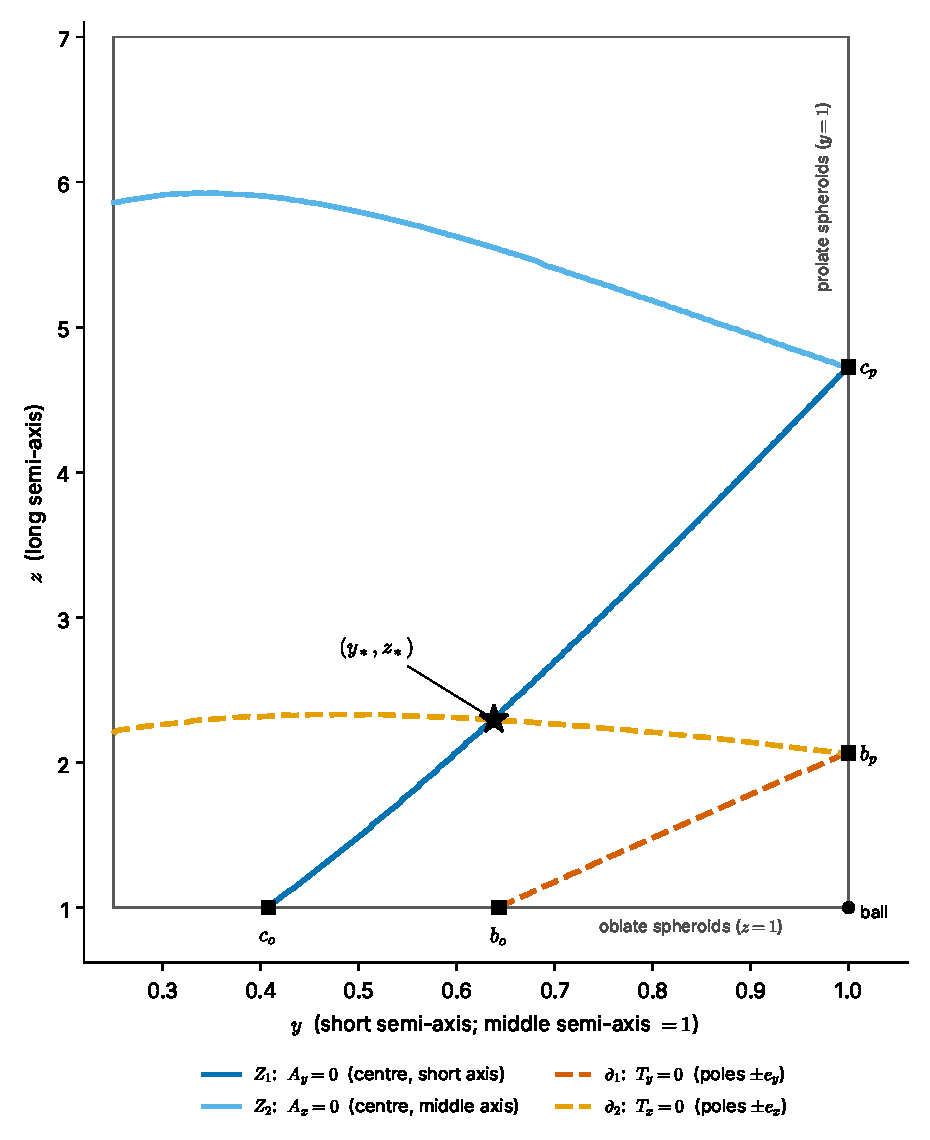
\includegraphics[width=0.78\textwidth,height=\textheight]{paper2_fig1_map.pdf}

\textbf{Figure 1.} The four zero curves in the rectangle R of shapes.
Solid: arcs from the centre (Z₁, Z₂). Dashed: arcs from the poles (∂₁,
∂₂). Squares: the four thresholds of {[}1{]} on the spheroid edges.
Star: the crossing point of Z₁ and ∂₂. The curves are drawn through the
centres of the certified strips and are an illustration; the statement
is Theorem 1.

\subsection{4 Theorem 2: what happens when a curve is crossed}

Theorem 1 locates four zero sets. Theorem 2 says that each of them is a
genuine threshold: when the shape crosses it, stationary points of the
energy enter or leave.

Nine further coefficients are needed. At the centre, \(A_{z}\) is the
curvature along the long axis and

\[
B_i=\tfrac16\,\partial_{q_i}^4E(0)\qquad(i=y,x).
\]

At the pole \(e_{i}\), \(N_{i}\) is the second radial derivative taken
from inside, and \(J_{ij}\) measures the curvature of E in a transverse
direction j:

\[
N_i=\partial_{q_i}^2E(e_i),\qquad \partial_{q_j}^2E(e_i)-T_i=(\ell_j^2-\ell_i^2)\,J_{ij}\qquad(j\ne i),
\]

where (\(\ell_{x}\), \(\ell_{y}\), \(\ell_{z}\)) = (1, y, z). The factor
\(\ell_{j}\)² − \(\ell_{i}\)² is taken out analytically, so \(J_{ij}\)
stays defined and continuous when two axes become equal.

\textbf{Theorem 2 (correspondence).} On R, the following strict signs
hold on the whole of each arc:

\begin{longtable}[]{@{}ll@{}}
\toprule\noalign{}
Arc & Certified signs \\
\midrule\noalign{}
\endhead
\bottomrule\noalign{}
\endlastfoot
Z₁ & \(A_{z}\) \textgreater{} 0, \(B_{y}\) \textless{} 0; and \(A_{x}\)
\textgreater{} 0 away from \(c_{p}\) \\
Z₂ & \(A_{z}\) \textgreater{} 0, \(B_{x}\) \textless{} 0; and \(A_{y}\)
\textless{} 0 away from \(c_{p}\) \\
∂₁ & \(N_{y}\) \textless{} 0, \(J_{yx}\) \textgreater{} 0, \(J_{yz}\)
\textgreater{} 0 \\
∂₂ & \(N_{x}\) \textless{} 0, \(J_{xy}\) \textgreater{} 0, \(J_{xz}\)
\textgreater{} 0 \\
\end{longtable}

Consequently the following hold. In parts 1, 2 and 4 the point of the
arc is not one of the shared end points \(c_{p}\), \(b_{p}\), and the
shape moves along a path in R that crosses the arc transversally there.
Part 3 concerns the shared end points, passed along the edge y = 1.

\begin{enumerate}
\def\labelenumi{\arabic{enumi}.}
\tightlist
\item
  \textbf{Centre (Z₁, Z₂).} In a neighbourhood of the centre, the
  stationary points other than the centre itself are exactly one pair ±r
  \(e_{i}\) on axis i on the side \(A_{i}\) \textgreater{} 0, and none
  on the side \(A_{i}\) \textless{} 0. The pair merges with the centre
  on the arc.
\item
  \textbf{Poles (∂₁, ∂₂).} In a neighbourhood of each pole ±\(e_{i}\),
  there is exactly one interior stationary point, on axis i, on the side
  \(T_{i}\) \textless{} 0, and none on the side \(T_{i}\) \textgreater{}
  0. On the arc the gradient trace vanishes at the pole itself.
\item
  \textbf{The symmetric edge.} At \(c_{p}\) and \(b_{p}\), which lie on
  the prolate edge y = 1, there is no pair: when the shape moves along
  the edge and passes \(c_{p}\) or \(b_{p}\), exactly one stationary
  circle in the equatorial plane enters or leaves, through the centre at
  \(c_{p}\) and through the equator of the boundary at \(b_{p}\).
\item
  \textbf{The crossing point.} At \((y_*, z_*)\) two independent events
  happen for the same shape: one at the centre on the short axis, one at
  the poles of the middle axis.
\end{enumerate}

On the map, the sides given by the theorem face each other: the
short-axis pair appears on the side of Z₁ that faces ∂₁ and on the side
of ∂₁ that faces Z₁, and likewise for the middle-axis pair between Z₂
and ∂₂. This suggests that each pair is born at the centre on its Z arc
and absorbed at the boundary on its ∂ arc. The suggestion agrees with
Paper I on both edges: on the oblate edge an axial pair exists for
\(c_{o}\) \textless{} λ \textless{} \(b_{o}\), and on the prolate edge a
stationary circle exists for \(b_{p}\) \textless{} λ \textless{}
\(c_{p}\).

Theorem 2 is local. It describes what enters or leaves near the centre
and near the poles when an arc is crossed. It does not count all
stationary points of a given shape, and it does not by itself show that
the pair persists throughout the region between its two arcs (Section
10).

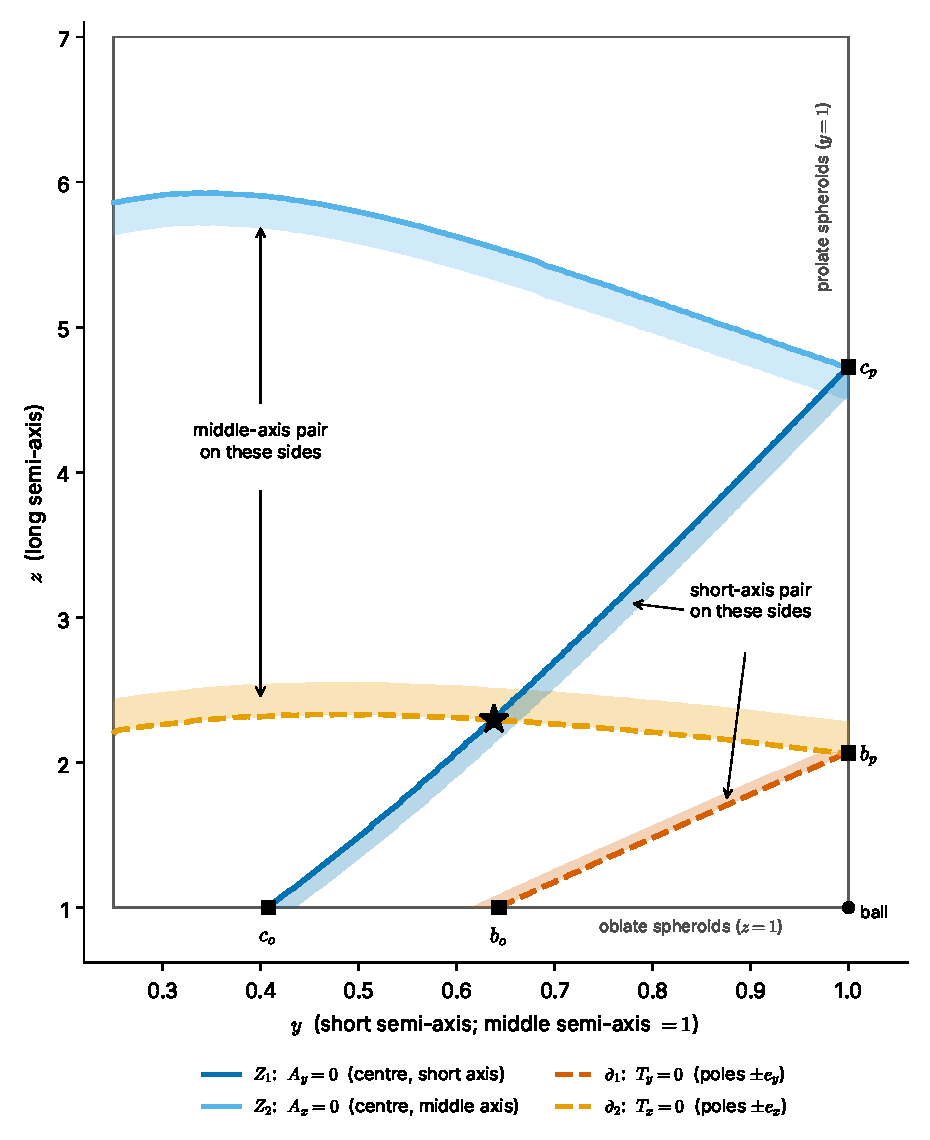
\includegraphics[width=0.78\textwidth,height=\textheight]{paper2_fig2_sides.pdf}

\textbf{Figure 2.} The side of each arc on which Theorem 2 places the
pair. The shaded band marks the side only; its width has no meaning.
Nothing is claimed about the regions between the arcs.

\subsection{5 Proof of Theorem 1}

Let H be one of \(A_{y}\), \(A_{x}\), \(T_{y}\), \(T_{x}\). All
enclosures below are rigorous intervals for H or a first derivative of H
over a whole shape box (Section 7). Rectangle coordinates are exact
rationals.

\textbf{Step 1: sign boxes.} R is subdivided into boxes. A box on which
the enclosure of H excludes zero is a sign box and contains no point of
the zero set. Sign boxes cover between 99.2\% and 99.8\% of the area of
R, depending on H.

\textbf{Step 2: strips.} A strip is a rectangle with a marked transverse
coordinate c ∈ \{y, z\} such that H is strictly negative on one of the
two faces c = const, strictly positive on the other, and
\(\partial_{c}\) H has a strict sign on the whole rectangle. On a strip,
for every value of the other coordinate there is exactly one zero of H,
so the zero set is the graph of a C¹ function and crosses the strip from
one end to the other. The strips number 276 (Z₁), 154 (Z₂), 111 (∂₁) and
71 (∂₂), plus one common strip for ∂₁ and ∂₂ at \(b_{p}\) (Step 4).

\textbf{Step 3: edges and connection.} On each edge of R the same method
in one variable gives sign intervals and root intervals with a strict
tangential derivative. This yields exactly two boundary roots for each
H, the ones listed after Theorem 1, and non-zero values at the four
corners. Consecutive strips overlap. Uniqueness in each strip does not
by itself show that the two graphs meet in the overlap, so this is
certified separately: for each pair of consecutive strips, and for each
end strip and its edge root, the ledger contains a segment inside the
overlap, transverse to the curve, with strictly opposite signs of H at
its two end points. By the intermediate value theorem H has a zero on
that segment; it belongs to both graphs, which therefore coincide on the
overlap. There are 618 such links, 610 between strips and 8 to edge
roots. The strips of each H form one chain that starts at one boundary
root and ends at the other.

\textbf{Step 4: the shared end points.} On the edge y = 1 the x and y
axes are equal, so \(A_{x}\) = \(A_{y}\) and \(T_{x}\) = \(T_{y}\)
there. Near such a point the two zero curves approach each other and
separate boxes for the two quantities cannot be told apart by
subdivision. Instead write, for H₁ = \(T_{y}\) and H₂ = \(T_{x}\),

\[
H_i(y,z)=P(z)-(1-y)\,M_i(y,z),\qquad M_i=\int_0^1\partial_yH_i\bigl(1-\theta(1-y),z\bigr)\,d\theta ,
\]

where P is the common value on the edge. Then H₁ − H₂ = (1 − y) D with D
= M₂ − M₁, and D is enclosed by the difference of the two
\(\partial_{y}\) enclosures over a window W around the point. No
division by 1 − y occurs. At \(b_{p}\) the window W = {[}31/32, 1{]} ×
{[}2, 17/8{]} gives D ∈ {[}−1.561, −0.067{]}, so the two curves do not
meet for y \textless{} 1 in W. A common strip {[}63/64, 1{]} × {[}2,
17/8{]} carries strict signs of both quantities on both faces and of
both \(\partial_{z}\) derivatives. The same argument at \(c_{p}\)
separates Z₁ and Z₂.

\textbf{Step 5: the remaining boxes.} After Steps 1--4, 8,674 small
boxes remained undecided. 242 strips are extended sideways, each in its
transverse direction, to a longer rectangle on which \(\partial_{c}\) H
keeps the same strict sign. The face signs of the original strip then
propagate to the extended rectangle, and the only zeros in it are those
on the original graph. With these 242 extensions and the common strip at
\(b_{p}\), every undecided box is contained in a finite union of
certified rectangles. This completes the cover: every point of R lies in
a sign box or in a rectangle whose zeros lie on the chain of Step 3.
Part 1 of the theorem follows.

\textbf{Step 6: pairs of curves.} A common zero of two quantities must
lie in the intersection of a strip of one with a strip of the other. All
such intersections are listed.

\begin{itemize}
\tightlist
\item
  Z₁, Z₂ and ∂₁, ∂₂: every overlap lies in the window of Step 4, where
  the only common point is the end point. This gives part 2.
\item
  Z₁, ∂₁; Z₂, ∂₁; Z₂, ∂₂: there is no overlap. This gives part 3.
\item
  Z₁, ∂₂: there are exactly four overlaps, all contained in the box
\end{itemize}

\[
X=[161/256,\,165/256]\times[291/128,\,37/16].
\]

\textbf{Step 7: the crossing in X.} Near X, Z₁ runs steeply (it is a
graph y = φ(z)) while ∂₂ is nearly horizontal (a graph z = ψ(y)). Put F
= \(A_{y}\) and G = \(T_{x}\). Over a box containing X the first
derivatives satisfy

\[
\begin{aligned}F_y&\in[0.7337,\,2.0574],&\quad F_z&\in[-0.3106,\,-0.1393],\\ G_y&\in[-0.2678,\,0.1208],&\quad G_z&\in[-0.2338,\,-0.1595].\end{aligned}
\]

The face signs of three Z₁ strips and two ∂₂ strips are carried to the
faces of X using \(F_{y}\) \textgreater{} 0 and \(G_{z}\) \textless{} 0:
F \textless{} 0 on the left face and F \textgreater{} 0 on the right
face; G \textgreater{} 0 on the bottom face and G \textless{} 0 on the
top face. By the Poincaré--Miranda theorem, F and G have a common zero
in X. If there were two, the mean value theorem along the two graphs
would give \textbar y − y′\textbar{} ≤ L₁ L₂ \textbar y − y′\textbar,
where L₁ and L₂ bound the slopes of φ and ψ, with

\[
L_1L_2\le\frac{\max|F_z|}{\min F_y}\cdot\frac{\max|G_y|}{\min|G_z|}\le 0.7105<1,
\]

a contradiction. (The bound 0.7105 is computed from the exact rational
end points; the display above shows them rounded outwards.) The same
bound shows that the Jacobian determinant is non-zero, so the crossing
is transversal. A Krawczyk test on the box {[}653/1024, 327/512{]} ×
{[}37619/16384, 37635/16384{]} ⊂ X, with contraction factor at most
0.0674 and image strictly inside the box, confirms the zero
independently and gives the enclosure of \((y_*, z_*)\) in part 4. ∎

\subsection{6 Proof of Theorem 2}

\textbf{Proposition C (centre).} Let p₀ be a shape with \(A_{i}\)(p₀) =
0 for i = y or x. Assume that \(A_{i}\) has non-zero derivative across
its zero set at p₀, that \(B_{i}\)(p₀) ≠ 0, and that \(A_{j}\)(p₀) ≠ 0
for the other two axes j. Then for shapes near p₀ the stationary points
near the centre, other than the centre, are exactly one pair ±r
\(e_{i}\) on the side \(A_{i}\) \(B_{i}\) \textless{} 0, and none on the
other side.

\emph{Proof.} Write Eᵢ and Eⱼ for the partial derivatives of E in qᵢ and
qⱼ. E is even in qᵢ, so on the axis Eᵢ(r eᵢ) = r H(r², p) with H
analytic (in this proof H is this function, not one of the four
quantities), H(0, p) = Aᵢ(p), and the derivative of H in its first
argument at (0, p₀) equal to Bᵢ(p₀). The implicit function theorem gives
one solution u(p) of H = 0 near u = 0, with the sign of −Aᵢ/Bᵢ. It gives
two points ±√u eᵢ when u \textgreater{} 0 and none when u \textless{} 0.
For j ≠ i, evenness gives Eⱼ = qⱼ Vⱼ with Vⱼ(0, p₀) = Aⱼ(p₀) ≠ 0, so
every nearby stationary point has qⱼ = 0. ∎

\textbf{Proposition P (pole).} Let p₀ be a shape with \(T_{i}\)(p₀) = 0.
Assume that \(T_{i}\) has non-zero derivative across its zero set at p₀,
that \(N_{i}\)(p₀) ≠ 0, and that \(\partial^2_{q_j}\)E(\(e_{i}\)) ≠ 0
for the other two axes j. Then for shapes near p₀ there is exactly one
interior stationary point near each pole ±\(e_{i}\) on the side
\(T_{i}\) \(N_{i}\) \textgreater{} 0, on the axis, and none on the other
side.

\emph{Proof.} Put Φ(d, p) = Eᵢ((1 − d)eᵢ) for d ≥ 0. Then Φ(0, p) =
Tᵢ(p), and the d-derivative of Φ at (0, p₀) is −Nᵢ(p₀). The inner
Hessian of E extends continuously to the closed ball (below), so this
derivative keeps a strict sign near (0, p₀), and Φ(d, p) = 0 has exactly
one solution d \textgreater{} 0 when Tᵢ Nᵢ \textgreater{} 0 and none
when Tᵢ Nᵢ \textless{} 0. For j ≠ i, the quotient Eⱼ/qⱼ is an average of
the second derivative Eⱼⱼ along a segment and tends to Eⱼⱼ(eᵢ) ≠ 0, so
nearby stationary points lie on the axis. ∎

\textbf{Regularity at the boundary.} With h = \textbar ξ − q\textbar{}
one has D ≥ y h and k ≤ h, hence \textbar{}\(\partial^2_{q}\)(k
f(g))\textbar{} ≤ C/h with C uniform on R. The function 1/h is
integrable on the sphere uniformly in q, so the inner Hessian is
continuous up to the boundary. (A numerical experiment at one shape
suggests that the second radial derivative approaches \(N_{i}\) no
faster than d log d.~This is an observation, not a proved statement, and
it is not used.) Proposition P uses continuity only. In more detail:
write v = q/\textbar q\textbar; then h² = (1 − \textbar q\textbar)² +
\textbar q\textbar{} \textbar ξ − v\textbar², so for
\textbar q\textbar{} ≥ 1/2 the integral of 1/h over a spherical cap of
radius ε around the pole is O(ε), uniformly in q; outside the cap the
integrand converges uniformly as q tends to the pole. The constant C is
uniform in q, in the shape on R and in the direction of differentiation,
because D ≥ h/4 and B ≥ 1/49 on R, and shape derivatives do not change
the order of the bound. The full argument is Section 1 of the derivation
file of the correspondence bundle (DERIVATION.md at commit 04051b6; see
Data and code availability).

\textbf{The transverse factor.} Rotating the point \(e_{i}\) towards
\(e_{j}\), together with the sphere variable, gives

\[
\partial_{q_j}^2E(e_i)-T_i=(\ell_j^2-\ell_i^2)\,J_{ij},
\]

with an explicit integrand for \(J_{ij}\) that involves no division by
\(\ell_{j}\)² − \(\ell_{i}\)² (Appendix A). On the arc \(T_{i}\) = 0, so
\(\partial^2_{q_j}\)E(\(e_{i}\)) = (\(\ell_{j}\)² − \(\ell_{i}\)²)
\(J_{ij}\), which is non-zero whenever \(J_{ij}\) ≠ 0 and the two axes
differ.

\textbf{Checking the hypotheses on the arcs.}

\begin{itemize}
\tightlist
\item
  Transversality is part of Theorem 1: every strip carries a strict sign
  of the transverse derivative.
\item
  On Z₁ away from \(c_{p}\), \(A_{x}\) \textgreater{} 0; on Z₂ away from
  \(c_{p}\), \(A_{y}\) \textless{} 0. Indeed Z₁ ∩ Z₂ = \{\(c_{p}\)\},
  each arc minus \(c_{p}\) is connected, and near \(c_{p}\) the
  certified sign of (\(A_{y}\) − \(A_{x}\))/(1 − y) \textless{} 0 fixes
  the sign.
\item
  The nine coefficients \(A_{z}\), \(B_{y}\), \(B_{x}\), \(N_{y}\),
  \(N_{x}\), \(J_{yx}\), \(J_{yz}\), \(J_{xy}\), \(J_{xz}\) are enclosed
  on all 614 strips (the 612 strips of Step 2 of Section 5, and the
  common rectangle at \(b_{p}\), which is recorded twice, once for ∂₁
  and once for ∂₂). A first pass over each whole strip settles 1,110 of
  the 1,412 strip--coefficient pairs. For the other 302, the strip is
  narrowed onto the true graph by an interval Newton step in the
  transverse direction, using the certified transverse derivative, and
  its base is bisected where needed. All 1,751 final pieces carry the
  strict sign stated in Theorem 2. No sign reversal and no zero of a
  coefficient occurs.
\item
  For ∂₁: \(\ell_{x}\)² − \(\ell_{y}\)² = 1 − y² \textgreater{} 0 for y
  \textless{} 1 and \(\ell_{z}\)² − \(\ell_{y}\)² \textgreater{} 0. For
  ∂₂: \(\ell_{y}\)² − \(\ell_{x}\)² = y² − 1 \textless{} 0 for y
  \textless{} 1 and \(\ell_{z}\)² − \(\ell_{x}\)² = z² − 1
  \textgreater{} 0, since ∂₂ does not reach z = 1.
\end{itemize}

With \(B_{i}\) \textless{} 0 the side \(A_{i}\) \(B_{i}\) \textless{} 0
is \(A_{i}\) \textgreater{} 0, and with \(N_{i}\) \textless{} 0 the side
\(T_{i}\) \(N_{i}\) \textgreater{} 0 is \(T_{i}\) \textless{} 0. This
gives parts 1 and 2.

\textbf{The symmetric edge (part 3).} At y = 1 the energy is invariant
under rotations about the z axis. At \(c_{p}\) both \(A_{x}\) and
\(A_{y}\) vanish; since \(A_{z}\) ≠ 0, nearby stationary points lie in
the plane \(q_{z}\) = 0, and Proposition C applied to H(u, p) with u =
\(q_{x}\)² + \(q_{y}\)² gives one stationary circle on the side
\(A_{i}\) \(B_{i}\) \textless{} 0 along the edge. At \(b_{p}\) the
tangential curvature at the pole vanishes by symmetry, and the one-sided
argument of Proposition P, applied in the equatorial plane, gives one
interior stationary circle on the side \(T_{i}\) \(N_{i}\)
\textgreater{} 0. On this edge the body is a prolate spheroid with axis
ratio λ = z, the two quantities reduce to the one-variable functions of
{[}1{]}, and the two statements are the events at \(c_{p}\) and
\(b_{p}\) found there: the stationary circle exists for \(b_{p}\)
\textless{} λ \textless{} \(c_{p}\). Part 3 adds nothing new on the
edge; it records that the pair of parts 1 and 2 becomes this circle when
the two axes become equal.

\textbf{The crossing point (part 4).} At \((y_*, z_*)\) the hypotheses
of Proposition C hold for i = y and those of Proposition P for i = x.
The two events take place at different points of the ball and are read
independently. ∎

\subsection{7 Computation and verification}

\textbf{Enclosing an integral over a shape box.} Each quantity is an
integral over a fixed square of two angular variables (Appendix A). The
integrand is evaluated with Taylor models in the two shape variables and
the angular variables, in MPFR interval arithmetic with outward rounding
at 128 bits; some edge evaluations in v1 and v2 were repeated at 256
bits. Each angular cell uses the two-point Gauss rule in each direction
with the signed remainder

\[
S\,Q_1Q_2G+\frac{S}{4320}\bigl(d_1^4[\partial_1^4G]+d_2^4[\partial_2^4G]\bigr),
\]

where S is the cell area, d₁ and d₂ its side lengths, and the brackets
are enclosures over the cell and over the whole shape box. The result is
intersected with the natural enclosure. The function f = arccos² and its
derivatives are enclosed by the series in 1 − g with 96 terms and an
explicit geometric tail. In v1 to v4 the angular grid is refined in
stages; 4,096 cells is the upper limit, reached only in the operations
that need it. Run C scans each strip with 64 and then 256 cells; where a
sign is still open it first narrows the strip onto the graph (Section 6)
and then evaluates with 1,024 cells.

\textbf{Ledgers.} Every evaluation is written to a ledger with its box
in exact rationals, its precision, its cell count and its interval. Sign
boxes, strips, edge roots, links between strips, extensions and
intersections are separate records that refer to evaluations by
identifier.

\textbf{Checkers.} Each run comes with a checker that takes the stored
integral enclosures as given and rebuilds every decision from their
rational end points: signs, the tiling of R by exact area, strip
conditions, links, the cover of the remaining boxes, the list of
overlaps, the Miranda and slope conditions, and the Krawczyk image. No
checker recomputes an integral. The checker of run C replays the stored
intervals through the same decision function that the producer used; for
that run the signs and the narrowing steps were therefore also
recomputed by the auditor with a separate implementation (below).

\textbf{Runs.} All runs were made on one machine (AMD Ryzen 9 9900X,
Ubuntu, GCC 15.2.0, MPFR 4.2.2, GMP 6.3.0). The plan and the code of
each run were fixed in a commit and audited before execution.

\begin{longtable}[]{@{}
  >{\raggedright\arraybackslash}p{(\columnwidth - 8\tabcolsep) * \real{0.2000}}
  >{\raggedright\arraybackslash}p{(\columnwidth - 8\tabcolsep) * \real{0.2000}}
  >{\raggedleft\arraybackslash}p{(\columnwidth - 8\tabcolsep) * \real{0.2000}}
  >{\raggedleft\arraybackslash}p{(\columnwidth - 8\tabcolsep) * \real{0.2000}}
  >{\raggedright\arraybackslash}p{(\columnwidth - 8\tabcolsep) * \real{0.2000}}@{}}
\toprule\noalign{}
\begin{minipage}[b]{\linewidth}\raggedright
Run
\end{minipage} & \begin{minipage}[b]{\linewidth}\raggedright
Purpose
\end{minipage} & \begin{minipage}[b]{\linewidth}\raggedleft
Cell evaluations
\end{minipage} & \begin{minipage}[b]{\linewidth}\raggedleft
Wall time
\end{minipage} & \begin{minipage}[b]{\linewidth}\raggedright
Outcome
\end{minipage} \\
\midrule\noalign{}
\endhead
\bottomrule\noalign{}
\endlastfoot
v2 & sign boxes, strips, edges, links & 93,135,344 & 4 h 5 min & four
chains complete; 8,674 boxes open \\
v3 & shared end points, strip extensions, pairs & 393,344 & 2 min 56 s &
cover complete; five of six pairs settled \\
v4 & crossing of Z₁ and ∂₂ & 8,160 & 4.5 s & main proof from existing
ledgers; Krawczyk confirms \\
C & nine coefficients on 614 strips & 4,405,328 & 9 min 36 s & all 1,412
strip--coefficient pairs strictly signed \\
\end{longtable}

The three numerical source files of the kernel are byte-identical in v1
to v4. Run C adds nine integrands to the same kernel and raises the
order of the derivative table of f from 8 to 9; the four original
integrands are unchanged.

\textbf{Independent audit.} Before each run an auditor checked the
derivation and the bundle, and after each run re-read the ledgers with
separate scripts that share no code with the producer. In particular:

\begin{itemize}
\tightlist
\item
  signs, exact area tiling, strip conditions and the cover of all 8,674
  remaining boxes were recomputed from the rational records;
\item
  the main proof of the crossing (Miranda, slope product, four overlaps
  in X) was confirmed from the frozen ledgers before v4 was executed,
  and the Krawczyk matrices, image and contraction factor were
  recomputed from the raw MPFR intervals;
\item
  the nine new coefficients were checked end to end at a sample shape
  against a direct numerical integration of the definition of E followed
  by finite differences in the position, without using the producer's
  formulas: seven digits for \(A_{z}\), \(B_{y}\), \(B_{x}\); three to
  four digits for the J coefficients; convergence to the kernel values
  for \(N_{y}\) and \(N_{x}\);
\item
  for run C, the transverse interval Newton steps of all 641 narrowed
  pieces were recomputed and matched exactly.
\end{itemize}

\textbf{What the proofs assume.} Correct rounding in MPFR 4.2.2; the
derivations of the integrands and remainders (Appendix A and the fixed
derivation files); the correctness of the kernel that turns these
formulas into the stored integral enclosures, which no checker
re-derives; and the correctness of the checkers, which are short and
public. The run records carry the grade DIAGNOSTIC\_ONLY; the results
were adopted by the author's rulings 2d2576e (Theorem 1; one end point
corrected in d6dc12b) and 8f9fe35 (Theorem 2) after the audits.

\subsection{8 GeoEnclosure at work: four runs with one kernel}

The proof of Theorem 1 was not reached in one step. We record the four
runs because the sequence shows what a certified enclosure can and
cannot do by itself, and what had to be added by design. The numerical
kernel was the same in all four; only the plan around it changed. This
section is a worked example of the GeoEnclosure methodology {[}2{]} on a
problem whose answer was not known beforehand; the same record, with the
reproduction code, is kept as an example in the GeoEnclosure repository
(Data and code availability).

\begin{longtable}[]{@{}
  >{\raggedright\arraybackslash}p{(\columnwidth - 10\tabcolsep) * \real{0.1667}}
  >{\raggedright\arraybackslash}p{(\columnwidth - 10\tabcolsep) * \real{0.1667}}
  >{\raggedleft\arraybackslash}p{(\columnwidth - 10\tabcolsep) * \real{0.1667}}
  >{\raggedleft\arraybackslash}p{(\columnwidth - 10\tabcolsep) * \real{0.1667}}
  >{\raggedright\arraybackslash}p{(\columnwidth - 10\tabcolsep) * \real{0.1667}}
  >{\raggedright\arraybackslash}p{(\columnwidth - 10\tabcolsep) * \real{0.1667}}@{}}
\toprule\noalign{}
\begin{minipage}[b]{\linewidth}\raggedright
Run
\end{minipage} & \begin{minipage}[b]{\linewidth}\raggedright
Plan
\end{minipage} & \begin{minipage}[b]{\linewidth}\raggedleft
Cell evaluations
\end{minipage} & \begin{minipage}[b]{\linewidth}\raggedleft
Wall time
\end{minipage} & \begin{minipage}[b]{\linewidth}\raggedright
What was certified
\end{minipage} & \begin{minipage}[b]{\linewidth}\raggedright
What stayed open
\end{minipage} \\
\midrule\noalign{}
\endhead
\bottomrule\noalign{}
\endlastfoot
v1 & sign boxes, with edge roots and strips attempted; fixed budget &
about 4 million & 9 min 5 s & sign on 1.5 \% to 16.8 \% of the area of
R, depending on the quantity & everything near the four curves \\
v2 & adaptive sign boxes, strips, edge roots, links & 93.1 million & 4 h
5 min & four complete chains of strips from edge to edge & 8,674 boxes;
the two shared end points; all six pairs \\
v3 & the factor 1 − y taken out at the shared end points; strip
extensions; pair windows & 393 thousand & 2 min 56 s & no box left open;
five of six pairs & the pair Z₁, ∂₂ \\
v4 & Miranda and slope product on existing ledgers; one Krawczyk step &
8,160 & 4.5 s & exactly one transversal crossing & nothing inside R \\
\end{longtable}

Three observations.

\begin{enumerate}
\def\labelenumi{\arabic{enumi}.}
\tightlist
\item
  \textbf{More computation did not close the proof.} v2 used about 23
  times as many cell evaluations as v1 and still left 8,674 boxes
  undecided. All of them were covered later by extended strips and the
  common strip (Step 5 of Section 5), that is, by a different statement.
  No refinement can give a strict sign on a box that meets the zero set.
\item
  \textbf{Each gap was closed by a change of statement, not of
  precision.} At the shared end points the two quantities agree
  identically on the edge y = 1, so the question was changed to the sign
  of D, the difference with the factor 1 − y taken out analytically.
  Next to the strips the question was changed from the sign of the
  quantity on a box to the sign of its transverse derivative on an
  extended strip: once that derivative keeps a strict sign on the whole
  extended strip, the signs already obtained on the faces of the
  original strip carry outwards. For the last pair the question was
  changed from disjointness to existence and uniqueness of one crossing.
  After each change the kernel answered at once: v3 and v4 together cost
  about 0.4 \% of the cells of v2.
\item
  \textbf{A failed attempt was kept in the record.} In v3 two attempts
  at the crossing failed. The auxiliary strips of v3 were taken with z
  as the transverse direction, and in the first Z₁ interval their face
  signs could not be settled, so the attempt stopped there; v4 treats Z₁
  as a graph y = φ(z) instead. The Krawczyk test was tried on three
  boxes at three grid stages each: on two boxes the contraction factor
  exceeded 1, and on the third it fell below 1 but the image was not
  strictly inside the box. The failure, its diagnosis and the corrected
  plan are all in the public ledgers.
\end{enumerate}

The limits are equally plain. The kernel proves strict inequalities on
boxes and nothing else; every topological conclusion in this paper comes
from an argument written by hand in Sections 5 and 6 and checked against
the ledgers. The region R, the choice of strips and the windows were
chosen by people and machines looking at uncertified pictures first.
GeoEnclosure is in this sense a heuristic methodology for finding a
proof: it does not tell which statement to certify, and it gives no
guarantee that a proof will close. What is guaranteed is only the
conclusion once it has closed. This section records one case; it is not
a claim of general effectiveness, and no comparison with other methods
of rigorous computation has been made.

\subsection{9 Relation to earlier work}

\textbf{Paper I.} The angle energy and its stationary points on
spheroids were treated in {[}1{]}. In the present coordinates the
spheroids are the two edges z = 1 (oblate) and y = 1 (prolate) of the
shape map, and the four thresholds of {[}1{]} are the four points
\(c_{o}\), \(b_{o}\), \(b_{p}\), \(c_{p}\) on these edges. Theorem 1
says how these four points are joined inside R: \(c_{o}\) to \(c_{p}\)
by Z₁, \(b_{o}\) to \(b_{p}\) by ∂₁, while Z₂ and ∂₂ leave \(c_{p}\) and
\(b_{p}\) and reach the edge y = 1/4. The stationary circles of {[}1{]}
reappear here as the degenerate case on the edge y = 1 (Section 6). The
classification in {[}1{]} is conditional on six computational assertions
stated there. Theorems 1 and 2 do not depend on them: the roots on the
edges of R are certified here independently, and {[}1{]} is used only to
identify them with its thresholds.

\textbf{Functionals of an interior point.} Points of a convex body
defined by extremising an integral of a function of the radial function
have been studied as radial centres {[}4{]}. The angle energy is a
functional of the same general kind, with the angle between the radial
direction and the normal as the integrand. We use no result from that
literature.

\textbf{Bifurcations in families of convex bodies.} Domokos, Holmes and
Lángi {[}3{]} classify convex solids by the equilibria of the distance
from a reference point and study how these equilibria change in one- and
two-parameter families through local and global bifurcations of gradient
vector fields. The present paper is a much narrower statement of the
same type for a different function: one two-parameter family, one
energy, and a certified location of the four curves on which a pair of
stationary points enters or leaves at the centre or at a pole.

\textbf{Computer-assisted proof.} The tools are standard: interval
arithmetic with correct rounding {[}8{]}, verification methods as
surveyed in {[}7{]}, the Poincaré--Miranda theorem {[}6{]} and the
Krawczyk operator {[}5{]}. Following a branch of zeros with rigorous
error bounds is a developed subject; see {[}9{]}. Our strips are a
simple form of this, adapted to an integrand that is expensive to
enclose. The organisation of the computation into a fixed plan, ledgers
and an independent checker follows {[}2{]}.

We did not find the configuration of Theorem 1 in the literature we
consulted, and we make no claim that the search was complete.

\subsection{10 Scope and open problems}

\textbf{What is proved.} Theorem 1 gives the position of the four zero
sets inside R = {[}1/4, 1{]} × {[}1, 7{]}. Theorem 2 gives the local
meaning of each arc: on crossing it transversally, exactly one pair of
stationary points appears or disappears in a neighbourhood of the centre
or of a pair of poles, on the stated side; at the shared end points
\(c_{p}\) and \(b_{p}\), passed along the edge y = 1, one stationary
circle appears or disappears instead.

\textbf{What is not proved.}

\begin{itemize}
\tightlist
\item
  \emph{Outside R.} Nothing is claimed for y \textless{} 1/4 or z
  \textgreater{} 7. Two arcs leave R through the edge y = 1/4; where
  they go is open.
\item
  \emph{The number of stationary points in each region.} The four arcs
  cut R into regions. Theorem 2 controls only what happens near the
  centre and near the two poles on the axes concerned. A count of all
  stationary points in a region needs, in addition, conditions of the
  following strength: that there is no stationary point at all off the
  plane \(q_{z}\) = 0, that in this plane none lies off the two axes,
  and a monotonicity along each axis which allows at most one pair on
  it. These global conditions have been formulated in the project record
  but are not used and not proved here.
\item
  \emph{Persistence.} That the pair created on an arc survives until the
  next arc is suggested by uncertified pictures only.
\item
  \emph{The nature of the stationary points.} We do not determine
  indices (saddle, maximum, minimum) of the points created.
\end{itemize}

\textbf{Assumptions.} The proofs rest on correct rounding in MPFR, on
the derivations of the integrands and their remainders, on the kernel
that computes the integral enclosures, and on the checkers (Section 7).

\textbf{Open problems.}

\begin{enumerate}
\def\labelenumi{\arabic{enumi}.}
\tightlist
\item
  Extend the map beyond R, in particular follow Z₂ and ∂₂ below y = 1/4.
\item
  Prove the global conditions and obtain the number of stationary points
  in each region of the map.
\item
  Give a proof of the single crossing of Z₁ and ∂₂ that does not use a
  computer, or an explanation of why the two curves must cross.
\item
  Decide whether the same four-curve picture holds for other energies
  built from the angle between the radial direction and the normal.
\end{enumerate}

\subsection{Process and AI disclosure}

This work was carried out by one human author together with several AI
systems, under a fixed division of roles. The author set the questions,
approved every plan before it was run, ruled on the adoption of every
result, and is responsible for the content.

\begin{itemize}
\tightlist
\item
  \textbf{ChatGPT (OpenAI)} operated the research computer, ran the
  fixed bundles and registered the results.
\item
  \textbf{ChatGPT Work (Astra, Codex)} wrote the plans, the derivations
  of the integrands and the code of the kernel, the producers and the
  checkers. It also reviewed draft v0.1 against the derivations and the
  code.
\item
  \textbf{Claude (Anthropic)} audited each derivation and bundle before
  the run and each result after it, with independent scripts, and
  drafted this manuscript.
\item
  \textbf{Claude Code (Anthropic)} reviewed the survey of earlier work
  and formulated the global conditions mentioned in Section 10. It
  reviewed draft v0.1 of this manuscript against the ledgers, the
  published version of {[}1{]}, the references and the cited commits; it
  read the ledgers and did not recompute any interval. It also built the
  interactive viewer, which Claude audited against the ledger and the
  text of this paper.
\item
  \textbf{Muse} (Meta), which took no part in the work, audited draft
  v0.1 of this manuscript for gaps in the line of proof and for
  overstatement. It found no gap in the proofs and asked for corrections
  of presentation, which are incorporated. It then audited the parts of
  Sections 4 to 6 that had changed in draft v0.5, including the argument
  for the connection of strips added after the review by Astra, and
  found nothing further to correct. It did not recompute anything.
\end{itemize}

Each plan, audit, approval and ruling is a dated commit in the public
repositories. No AI system is an author. The author read the complete
manuscript in a Japanese translation of this text and approved it on 27
November 2026.

\subsection{Data and code availability}

All material is public and pinned by commit. Repository of this paper:
\url{https://github.com/cotaxxxx/bg-triaxial-family}

\begin{longtable}[]{@{}
  >{\raggedright\arraybackslash}p{(\columnwidth - 2\tabcolsep) * \real{0.3429}}
  >{\raggedright\arraybackslash}p{(\columnwidth - 2\tabcolsep) * \real{0.6571}}@{}}
\toprule\noalign{}
\begin{minipage}[b]{\linewidth}\raggedright
Item
\end{minipage} & \begin{minipage}[b]{\linewidth}\raggedright
Commit
\end{minipage} \\
\midrule\noalign{}
\endhead
\bottomrule\noalign{}
\endlastfoot
Derivation of the four integrands &
\texttt{f8c809f2e2cfdc32da04aba120e7e8fd1001de7e} \\
Bundle v2 & \texttt{bb50c85c1bff93e3e04b54c5cbd218dcb3768a96} \\
Bundle v3 & \texttt{cdd885b5ff0fa31408f08a97c382f230f24bab04} \\
Bundle v4 & \texttt{e7c039ee315162a9d3e001734128023bba3ac00f} \\
Bundle C (correspondence) &
\texttt{04051b610bd1ada9992e8912a3bdad4954ae929c} \\
Result v1 & \texttt{e5456d8ca3966330f39ae0490ca1637d703c09c6} \\
Result v2 & \texttt{862220cc03f8044ab770548d865a76ed56fc612c} \\
Result v3 & \texttt{7c6cd7ecb21d7d4465e2140c5465412e4f3a4720} \\
Result v4 & \texttt{f58ca0c871bc075c89f09aa1df5a2e4ec4b702b7} \\
Result C & \texttt{5959680d898dee1289c4023e059dd7e5b84847cf} \\
Adoption of Theorem 1 &
\texttt{2d2576ee43f07a3cb94df28d63051f52649e3c81} \\
Correction of one end point &
\texttt{d6dc12b24a3a1b7575350cdd8bed7e24494eaa89} \\
Adoption of Theorem 2 &
\texttt{8f9fe35af8675f3e043d7849ba2ab065efcf6634} \\
Interactive viewer &
\texttt{202744a3074910df1b9e0bf9759144f24493ba56} \\
\end{longtable}

Bundle C is on the branch codex/paper-ii-correspondence-20261127 and the
viewer on the branch claude/paper-ii-viewer-20261127; they are not
reachable from the other branches. The audits, the rulings, the external
audits, the reviews and the responses to them are on the branch
evidence/triaxial-chat.

Record of the method as a worked example:
\url{https://github.com/cotaxxxx/GeoEnclosure}, directory
examples/triaxial-four-curves. Process records:
\url{https://github.com/cotaxxxx/experimental-mathematics-ai-collaboration}

A reproduction archive (the four bundles with their code and plans, the
result ledgers, the checkers, the independent audit scripts, the figure
script and the sources of the viewer, with SHA-256 sums and
instructions) is attached to the Zenodo record of this paper
(doi:10.5281/zenodo.24581453).

\textbf{Interactive viewer.} The Zenodo record also contains a linked
viewer of the map: one self-contained HTML file with no network access,
in English and Japanese. Choosing a shape on the map of Figure 1 shows
the corresponding ellipsoid and, when the shape lies in a certified
strip, the local event of Theorem 2. The viewer is built from the ledger
of run v2 by a script in the archive. It is an illustration and not part
of any proof. It can also display uncertified floating-point positions
of stationary points on the axes; this layer is off by default and is
labelled as not proved here.

\subsection{References}

{[}1{]} K. Furuta, \emph{Saddle pairs, a saddle circle, and nothing
else: stationary points of an angle energy across all spheroid shapes},
Version v1.0, Zenodo, 2026. doi:10.5281/zenodo.24495446

{[}2{]} K. Furuta, \emph{GeoEnclosure: A Methodology of Interval
Enclosure and Sign Determination Based on Problem Structure}, Version
1.0, Zenodo, 2026. doi:10.5281/zenodo.24421364

{[}3{]} G. Domokos, P. Holmes, Z. Lángi, A genealogy of convex solids
via local and global bifurcations of gradient vector fields, \emph{J.
Nonlinear Sci.} 26 (2016), 1789--1815. doi:10.1007/s00332-016-9319-4

{[}4{]} I. Herburt, M. Moszyńska, Z. Peradzyński, Remarks on radial
centres of convex bodies, \emph{Math. Phys. Anal. Geom.} 8 (2005),
157--172.

{[}5{]} R. Krawczyk, Newton-Algorithmen zur Bestimmung von Nullstellen
mit Fehlerschranken, \emph{Computing} 4 (1969), 187--201.
doi:10.1007/BF02234767

{[}6{]} C. Miranda, Un'osservazione su un teorema di Brouwer,
\emph{Boll. Un. Mat. Ital.} (2) 3 (1940), 5--7.

{[}7{]} S. M. Rump, Verification methods: rigorous results using
floating-point arithmetic, \emph{Acta Numerica} 19 (2010), 287--449.

{[}8{]} The GNU MPFR Library, version 4.2.2. https://www.mpfr.org

{[}9{]} J. B. van den Berg, J.-P. Lessard, K. Mischaikow, Global smooth
solution curves using rigorous branch following, \emph{Math. Comp.} 79
(2010), 1565--1584. doi:10.1090/S0025-5718-10-02325-2

\subsection{Appendix A. The integrands}

This appendix lists the formulas that the kernel encloses. Throughout, ℓ
= (1, y, z) are the semi-axes in the order (x, y, z), \(h_{l}\) =
\(\ell_{l}\)², and f = arccos². The symbol B without an index is the
quadratic form of Section 2; B with an index is the fourth-order
coefficient of Section 4. Full derivations, with the exact rational spot
checks made before the runs, are in the fixed derivation files (Data and
code availability).

\subsubsection{\texorpdfstring{A.1 Centre curvature
\(A_{i}\)}{A.1 Centre curvature A\_\{i\}}}

At q = 0 put \(S_{j}\) = \(\xi_{j}\)² and

\[
d=\sum_j \ell_j^2 S_j,\qquad B=\sum_j \ell_j^{-2}S_j,\qquad U_i=\ell_i^2/d,\qquad g_0=(dB)^{-1/2}.
\]

Differentiating k f(g) twice in \(q_{i}\) under the integral gives the
integrand

\[
\mathcal A_i=g_0^2 f''(g_0)\,S_i\,(U_i-1)^2+g_0 f'(g_0)\bigl[S_i(3U_i^2-4U_i+2)-U_i\bigr].
\]

It depends only on the squares \(S_{j}\). With the marked axis i as
polar axis, μ = \(\xi_{i}\), \(S_{i}\) = μ², \(S_{m}\) = (1 − μ²) cos²φ,
\(S_{n}\) = (1 − μ²) sin²φ and φ = πw/2,

\[
A_i(y,z)=\int_0^1\!\!\int_0^1 \mathcal A_i(\mu,w;y,z)\,d\mu\,dw .
\]

The bounds d ≥ y², B ≥ z⁻² and

\[
dB=1+\sum_{j<k}S_jS_k\bigl(\ell_j/\ell_k-\ell_k/\ell_j\bigr)^2\ \ge 1
\]

keep g₀ in (0, 1{]}.

\subsubsection{\texorpdfstring{A.2 Pole trace
\(T_{i}\)}{A.2 Pole trace T\_\{i\}}}

For fixed ξ,

\[
\partial_{q_i}\bigl(k f(g)\bigr)=-\xi_i\,(f+g f')+\frac{k\,\ell_i^2(\xi_i-q_i)}{D^2}\,g f' .
\]

The right side is bounded uniformly on compact sets of shapes, so the
limit q → \(e_{i}\) may be taken under the integral. At q = \(e_{i}\)
put μ = \(\xi_{i}\) = 1 − 2r² with 0 ≤ r ≤ 1, so that k = 2r², and

\[
\begin{aligned}
d_i&=(1-r^2)(\ell_m^2\cos^2\varphi+\ell_n^2\sin^2\varphi)+r^2\ell_i^2,\\
B_i^{\ast}&=\mu^2/\ell_i^2+4r^2(1-r^2)(\ell_m^{-2}\cos^2\varphi+\ell_n^{-2}\sin^2\varphi),\\
g^{\ast}&=r/\sqrt{d_iB_i^{\ast}} .
\end{aligned}
\]

Then D² = 4r² \(d_{i}\), the factor r² cancels, and

\[
\mathcal T_i=-\mu\bigl(f(g^{\ast})+g^{\ast}f'(g^{\ast})\bigr)-\frac{\ell_i^2r^2}{d_i}\,g^{\ast}f'(g^{\ast}),\qquad
T_i(y,z)=\int_0^1\!\!\int_0^1 2r\,\mathcal T_i\,dr\,dw .
\]

Only the positive quantities \(d_{i}\) and \(B_{i}^{\ast}\) are divided
by, also at the point of contact r = 0.

\subsubsection{\texorpdfstring{A.3 Fourth-order centre coefficient
\(B_{i}\)}{A.3 Fourth-order centre coefficient B\_\{i\}}}

Along the axis i write q = t \(e_{i}\). Then k = 1 − μt and D(t)²/D(0)²
= 1 − 2Uμt + Ut² with U = \(h_{i}\)/d.~Let

\[
\begin{gathered}(1-2U\mu t+Ut^2)^{-1/2}=\sum_{n\ge0}\eta_n t^n,\\ n\,\eta_n=(2n-1)U\mu\,\eta_{n-1}-(n-1)U\,\eta_{n-2},\qquad \eta_0=1 .\end{gathered}
\]

Then g(t) = g₀ + δ(t) with δ(t) = Σ \(g_{n}\) tⁿ, \(g_{n}\) =
g₀(\(\eta_{n}\) − μ \(\eta_{n-1}\)), and the integrand of \(B_{i}\) =
\(E_{iiii}\)(0)/6 over dμ dw is

\[
4\,[t^4]\Bigl\{(1-\mu t)\sum_{m=0}^{4}\frac{f^{(m)}(g_0)}{m!}\,\delta(t)^m\Bigr\}.
\]

\subsubsection{\texorpdfstring{A.4 Pole Hessian: \(N_{i}\) and
\(J_{ij}\)}{A.4 Pole Hessian: N\_\{i\} and J\_\{ij\}}}

Use the variables of A.2, write n = (ξ − \(e_{i}\))/(2r), so that
\(n_{i}\) = −r and \(n_{j}\)² = (1 − r²)cos²φ or (1 − r²)sin²φ, and put

\[
d=\sum_l h_l n_l^2,\qquad b=\sum_l \xi_l^2/h_l,\qquad P=(db)^{-1/2},\qquad g=rP .
\]

\emph{Radial coefficient.} With M = r \(h_{i}\)/d and U = −μP − gM, the
integrand of \(N_{i}\) = \(E_{ii}\)(\(e_{i}\)) over dr dw (area weight
2r included) is

\[
-2\mu\,f'(g)\,U+r\Bigl\{f''(g)\,U^2+f'(g)\bigl[2\mu PM+g\,(3M^2-h_i/d)\bigr]\Bigr\}.
\]

\emph{Transverse coefficient.} Rotating q and the sphere together in the
plane (\(e_{i}\), \(e_{j}\)) gives \(E_{jj}\)(\(e_{i}\)) − \(T_{i}\) = Δ
\(J_{ij}\) with Δ = \(h_{j}\) − \(h_{i}\). With η = −1/(\(h_{i}\)
\(h_{j}\)), p = r/d, t = 2ηrμ/b, V = t − p and

\[
W=\frac{r^2-n_j^2}{d}+\eta\,\frac{\mu^2-4r^2n_j^2}{b},
\]

the integrand of \(J_{ij}\) over dr dw is

\[
4r^3\Bigl\{\bigl(g^2f''(g)+g f'(g)\bigr)\,\Delta\,n_j^2\,V^2+g f'(g)\bigl[-W+2\Delta\,n_j^2\,(p^2+t^2)\bigr]\Bigr\}.
\]

No division by Δ occurs, so \(J_{ij}\) is defined and enclosed also
where two axes are equal.

\subsubsection{A.5 The function f and the quadrature remainder}

With b = 1 − g in {[}0, 1{]},

\[
f(g)=\sum_{n\ge1}c_n b^n,\qquad c_1=2,\qquad c_{n+1}=c_n\,\frac{n^2}{(n+1)(2n+1)} .
\]

All coefficients are positive. Derivatives are taken term by term; terms
up to n = 96 are summed and the tail is enclosed by 5/2 times the term n
= 97, which is valid for derivative orders up to 9 because the ratio of
consecutive differentiated terms is below 3/5 there.

On an angular cell with sides d₁, d₂ the two-point Gauss rule is exact
for cubics, and comparison with the cubic Hermite interpolant at the
nodes gives the one-dimensional remainder d⁴ G⁗/4320 for the normalised
integral. Applying it in each direction gives the enclosure displayed in
Section 7. Shape derivatives of all integrands are obtained by
differentiating the fixed-domain formulas above; they are bounded and
continuous, so they equal the derivatives of the integrals.

\subsection{Appendix B. Title and abstract in Japanese}

\begingroup\jafont\XeTeXlinebreaklocale ``ja''\XeTeXlinebreakskip=0pt
plus 1pt

\textbf{三軸楕円体の角度エネルギー地図 ―
停留点が出入りする四本の境目（再現コード・ビューア付き）}

凸体とその内部の一点に対して、その点から境界の点を見る向きと、そこでの外向き法線とがなす角の二乗を、錐体積の重みで平均したものを角度エネルギーと呼ぶ。回転楕円体でのこのエネルギーの停留点は、この連作の第一論文（論文
I、doi:10.5281/zenodo.24495446）で、そこに述べた六つの計算主張を条件として分類した。そこには四つの閾値の形が現れた。本論文は、三本の軸がすべて違う楕円体を扱う。半軸を
y ≤ 1 ≤ z と書き、形の長方形 R = {[}1/4, 1{]} × {[}1, 7{]}
の上で、最長軸以外の二本の軸それぞれについて、中心でのエネルギーの二階微分と、その軸の端でのエネルギーの動径方向の微分という、四つの量を考える。

R
の中で、四つの量それぞれの零集合は一本の弧である。四本の弧が出会うのは、辺
y = 1 の上の二つの扁長側の閾値の形と、内部のただ一点（横断的な交わり、y
≈ 0.6382、z ≈
2.2966）だけである。回転楕円体の四つの閾値はこれらの弧の端点で、残る二つの端は辺
y = 1/4
の上にある。さらに、各弧は次の局所的な意味で境目である。形が弧を横切るとき、エネルギーの停留点がちょうど一対、中心を通って、または向かい合う一対の極を通って出入りし、どちら側に対があるかも決まる。二つの扁長側の閾値の形では、形が辺
y = 1 に沿って動くとき、対の代わりに一つの停留円が出入りする。

証明は計算機を使い、GeoEnclosure
の方法論（doi:10.5281/zenodo.24421364）に従う。面積分を MPFR
の区間演算で囲み、有理数の台帳に記録し、数値のコードとは独立の検査器で確かめる。第一の主張の証明に至る四回の実行（v1〜v4）を、数値の核を変えないまま、GeoEnclosure
の一つの実例として記録する。この場合、証明は、精度を上げることによってではなく、確かめる命題を変えることによって閉じた。地図の各領域にある停留点の個数は、本論文では決めない。

\endgroup

\end{document}
